% LaTex Klasse
\documentclass[10pt,a4paper,article,oneside]{memoir}

%% Pakete default
\usepackage[utf8]{inputenc} 
\usepackage[backend=biber,bibencoding=utf8,sorting=nyt,language=ngerman, style=alphabetic]{biblatex}
\usepackage[breaklinks=true]{hyperref}
\usepackage[german]{babel}
\usepackage{graphicx}
%\usepackage{subfig}
\usepackage{subfloat}
\usepackage{eurosym}
\usepackage{amsmath}

\usepackage{xcolor}
\colorlet{shadecolor}{gray!25} 
\definecolor{darkblue}{rgb}{0,0,.5}
\hypersetup{linktocpage}
\hypersetup{ colorlinks=true, pdfborder={0 0 0},  urlcolor=darkblue} 

%% Pakete usefull
\usepackage{tikz}
\newsubfloat{figure}
% Command to set caption styles
\captionnamefont{\bfseries\small}
\captiontitlefont{\itshape\small}
\subcaptionlabelfont{\bfseries\small}
\subcaptionfont{\itshape\small}


%\usepackage{tikzscale}
%\usepackage{bbding}
%\usepackage{listings} 
%\usepackage{epstopdf}
%\usepackage{pgfgantt}
%\usepackage{wrapfig}
%\usepackage{mathtools}
%\usepackage[page]{appendix}

%% R\"omishce zeichen
%\newcommand{\rmnum}[1]{\romannumeral #1}

%%line space
\DisemulatePackage{setspace}
\usepackage{setspace}
%%set global linespace
\newcommand{\mylinespace}{1.2}

% Image floating
%\newcommand{\illustrationname}{Illustration}
%\newfloat[chapter]{illustration}{lol}{\illustrationname}

%% Absatzeinzug!!!
\setlength{\parindent}{0pt}

%% TiKz Stuff %%%
\usetikzlibrary{calc, decorations.pathmorphing,decorations.pathreplacing, fadings, shadings, shapes, arrows,trees, positioning,patterns,automata}
%\pgfdeclarelayer{background}
%\pgfdeclarelayer{foreground}
%\pgfsetlayers{background,main,foreground}
%\usepackage{tikz-uml}
%\usepackage{pgfplots}

%% Bib
\bibliography{references}
%\defbibheading{bibliography}{\bibsection}


%% PAGE DIMENSIONS A4  % This is from memman.pdf
\settrimmedsize{297mm}{210mm}{*}
\setlength{\trimtop}{0pt}
\setlength{\trimedge}{\stockwidth}
\addtolength{\trimedge}{-\paperwidth}
\settypeblocksize{670pt}{410pt}{*}
\setulmargins{3cm}{*}{*}
\setlrmargins{*}{*}{0.8}
\setmarginnotes{17pt}{51pt}{\onelineskip}
\setheadfoot{\onelineskip}{2\onelineskip}
\setheaderspaces{*}{2\onelineskip}{*}
\checkandfixthelayout

%\maketitle % CUSTOMISATION
 % to be done
 %\pagenumbering{Roman}

% For more than trivial changes, you may as well do it yourself in a titlepage environment 
 %\pretitle{\begin{center}\sffamily\huge\MakeUppercase}
 %\posttitle{\par\end{center}\vskip 0.5em}

%%% ToC (table of contents) APPEARANCE
 %\maxtocdepth{subsection} % include subsections
 %\renewcommand{\cftchapterpagefont}{}
 %\renewcommand{\cftchapterfont}{} % no bold!

%%% HEADERS & FOOTERS
\pagestyle{plain} % try also: empty , plain , headings , ruled , Ruled , companion

%%% CHAPTERS
\chapterstyle{section} %southall} % try also: default , section , hangnum , companion , article, demo

\renewcommand{\chaptitlefont}{\Huge\sffamily\raggedright} % set sans serif chapter title font
\renewcommand{\chapnumfont}{\Huge\sffamily\raggedright} % set sans serif chapter number font

%%% SECTIONS
\hangsecnum % hang the section numbers into the margin to match \chapterstyle{hangnum}
\maxsecnumdepth{subsection} % number subsections

\setsecheadstyle{\Large\sffamily\raggedright} % set sans serif section font
\setsubsecheadstyle{\large\sffamily\raggedright} % set sans serif subsection font


%% END Memoir customization

%% TikZ input Hack
 \newcommand{\inputTikZ}[1]{\input{#1.tikz}} 
 %\newsubfloat{figure} %% use for \subbottom or \subtop in a figure

%%%##########################################
% Content Composer
\newboolean{de}
\newboolean{fullfrontpage}


\setboolean{de}{true} %DE - true; EN - false
\setboolean{fullfrontpage}{true} % full - true; just a header - false

%set publisher
\newcommand{\docType}{Lab Report}
\newcommand{\docTypeRubric}{\glqq Strömungssimulation in der erweiterten Realität\grqq}
\newcommand{\docCourse}{Master Projekt System Entwicklung}
\newcommand{\docCourseSemester}{WS 2013/14}
\newcommand{\docCourseProf}{Prof. Dr. J. Wietzke, Prof. Dr. E. Hergenröther}
\newcommand{\docDate}{01.05.2013}
\newcommand{\docStudentA}{T. Sturm}
\newcommand{\docStudentAMatrikel}{709794}
\newcommand{\docStudentB}{A. Holike}
\newcommand{\docStudentBMatrikel}{724986}
\newcommand{\docStudentC}{S. Arthur}
\newcommand{\docStudentCMatrikel}{715720}
\newcommand{\docStudentD}{M. Djakow}
\newcommand{\docStudentDMatrikel}{718531}

%%% #########################################
%%% BEGIN DOCUMENT

\begin{document}

%Titel
\iffullfrontpage
	% !TEX root = ../report.tex
% begin title
\begin{titlingpage}
	\vspace*{0cm}
	\sffamily 
	\begin{centering}
		
\includegraphics[width=0.5\textwidth]{images/fbi_logo.pdf} \\
		\vspace{2.5cm}
		\Huge
			\textbf{\docType} \\
		\vspace{1cm}
		\normalsize
			\docCourse, \docCourseSemester \\
		\small
			(\textit{\docCourseProf}) \\
		\vspace{3cm}
		\LARGE
			\docTypeRubric \\
		\vspace{4cm}
		\normalsize
			\ifde
				%vorgelegt von\\
			\else
				%submitted by\\
			\fi
		\vspace{1cm}	
		\large
			\docStudentA, \docStudentB, \docStudentC, \docStudentD \\
			\vspace{1cm}
		\normalsize
			\docDate \hspace{1cm} Version: \docVersion \\
	\end{centering}
	
\end{titlingpage}

%% End Of Doc
\else
	% !TEX root = ../report.tex
% begin title
\begin{centering}
	\sffamily
	\vspace*{0.5cm}
	\huge
		\docType \\
	\vspace{0.5cm}
	\small
		\docCourse, \docCourseSemester \\
	\footnotesize
		(\textit{\docCourseProf}) \\
	\vspace{0.5cm}
		\large
			\docTypeRubric, \hspace{0.1cm} \docDate \\
		\vspace{0.5cm}
		\small
			\ifde
				vorgelegt von\\
			\else
				submitted by\\
			\fi
		\vspace{0.25cm}	
		\small
			\docStudentA \hspace{0.1cm} (\docStudentAMatrikel)\\
			\docStudentB  \hspace{0.1cm} (\docStudentBMatrikel)\\
		\vspace{0.5cm}
		
		\rule{12cm}{0.025cm}
		
\end{centering}
\vspace{1cm}
%% End Of Doc
\fi

\tableofcontents* % the asterisk means that the contents itself isn't put into the ToC

\clearpage %schreibt letztes Kapitel fertig, noetig fuer toc


%%% BEGIN  CONTENT %%%
%% Styles für TikZ
  %\include{graphics/styles}

% !TEX root = ../report.tex
\chapter{Einleitung}
\begin{Spacing}{\mylinespace}
\begin{figure}[h!]
	\centering
	\includegraphics[width=\textwidth]{graphics/intro.png}
	\vspace{20px}
\end{figure}
Die Technik der Strömungssimulation spielt heutzutage eine größere Rolle den je. Lange ist es her das Windkanäle nur zur Erforschung und Verbesserung der Aerodynamik von Flugzeugen genutzt wurden. Heute gibt es kaum noch ein Kraftfahrzeug das nicht im Windkanal optimiert wurde und auch Architekten und Statiker nutzen immer häufiger den Windkanal um ihre Konstruktionen und Berechnungen zu überprüfen. Ein relativ neues Thema in diesem Gebiet ist die Untersuchung von kompletten Stadtteilen und Städten im Windkanal. Durch den enormen Anstieg von neuen Wohn-, Gewerbe- und Industriegebieten in den letzten Jahrzehnten, schrumpft der Anteil von freien und natürlichen Flächen immer weiter, wodurch die Frischluftzufuhr negativ beeinflusst wird und sich das Klima in Städten stetig weiter erwärmt und verschlechtert. Um dieser Entwicklung entgegen zu wirken nutzen auch Städteplaner immer häufiger die Vorzüge des Windkanals.
\\\\
So nützlich der Windkanal auch für alle vorgestellten Anwendungen ist, so ist dessen Nutzung auch immer mit sehr hohen Kosten verbunden. Durch die immer weiter steigende Leistung von Computern liegt es deshalb nahe, zu versuchen, erste Tests und Untersuchung von der Realität auf den Computer auszulagern und auf diesem zu simulieren. Genau aus diesem Gebiet bestand der Hauptteil unserer Forschung in diesem Semester. Um dieses doch sehr mathematische und trockene Thema für Außenstehende noch etwas attraktiver und greifbarer zu machen haben wir es jedoch, mit Hilfe der Kinect Kamera von Microsoft, noch um eine Interaktive Komponente erweitert.
\\\\
Auf den Folgenden Seiten werden wir nun unser Vorgehen sowie die Fortschritte, Erfahrungen und Ergebnisse dieses Projekts vorstellen.
\end{Spacing}
\newpage
\clearpage
%% End Of Doc
\clearpage
% !TEX root = ../report.tex
\chapter{Bestehende Arbeiten}
\begin{Spacing}{\mylinespace}
\begin{figure}[h!]
	\centering
	\includegraphics[width=\textwidth]{graphics/relatedWork.png}
	\caption{(a) Augmented Reality Sandbox. (b) A Particle System
for Interactive Visualization of 3D Flows. (c) Synthetic Turbulence using Artificial Boundary Layers. (d) Scalable Fluid Simulation using Anisotropic Turbulence Particles}
	\label{fig:relatedWork}
\end{figure}
Bevor wir auf unsere eigene Arbeit eingehen, wollen wir kurz einige andere Arbeiten vorstellen die sich mit ähnlichen Themen beschäftigen und an denen wir uns zum Teil orientiert haben.
\\\\
Beginnen wollen wir mit der \textit{Augmented Reality Sandbox} \cite{Kre10} einem beeindruckenden Projekt der \textit{University of California} in Zusammenarbeit mit weiteren Forschungsinstituten, welches die Grundidee zu unserer Integrierung der Kinect 3D Kamera von Microsoft und dem Sandkasten lieferte. Ziel dieses Projekts war es, mit Hilfe der Kinect Kamera, eine spielerische Möglichkeit zu entwickeln, die es erlaubt topologische Landschaft, durch formen des Sandes mit den eigenen Händen, zu erstellen. Zusätzlich nutzen sie auch ein physikalisches System zur Simulation von Wasser die man in Abbildung \ref{fig:relatedWork} gut erkennen kann.
\\\\
Mit physikalischen System in Bezug auf Strömungssimulation beschäftigen sich auch die folgenden Arbeiten. \textit{A Particle System
for Interactive Visualization of 3D Flows} \cite{Kru05} ist zwar schon etwas älter, aber es ist eine der ersten Arbeiten in der mit der Auslagerung der Physikberechnung auf die GPU, um realistische Echtzeitströmungen zu simulieren, experimentiert wird. Zudem werden sehr interessante Konzepte genutzt, wie zum Beispiel die Speicherung der Partikelpositionen in einer Textur die gleichzeitig als Ein- und Ausgabecontainer zwischen den einzelnen Berechnungsschritten dient.
\\\\
Eine weitere interessante Arbeit ist \textit{Synthetic Turbulence using Artificial Boundary Layers} \cite{Pfa09}. Hier werden vorberechnete Strömungsfelder zur Simulation der Partikel genutzt um  extrem realistische Darstellungen zu realisieren. Durch die Vorberechnung verfügt dieses Verfahren aber leider über keine Echtzeitfähigkeit. In der Folgearbeit \textit{Scalable Fluid Simulation using Anisotropic Turbulence Particles} \cite{Pfa10} wird dieses Manko, durch starke Parallelisierung und der Berechnung vieler kleineren Einzelsimulationen, allerdings behoben.



\end{Spacing}
\newpage
\clearpage
%% End Of Doc
\clearpage
% !TEX root = ../report.tex
\chapter{Konzept}
\begin{Spacing}{\mylinespace}

Wie bereits in der Einleitung angeführt, soll eine Strömungssimulation erarbeitet werden. Die Grundlage hierfür bilden zwei optische System. Im ersten Teil wird die Oberfläche mit einer Tiefenkamera eingelesen. Der zweite Teil besteht aus einem Projektor, welcher die simulierte Strömung direkt auf die eingelesene Oberfläche projiziert. Dies soll in Echtzeit erfolgen. Als Kernstück soll mit einem Rechner gearbeitet werden, auf dem die Simulationssoftware ausgeführt wird und alle optischen Systeme angebunden sind.

\section{Der Datenfluss}
Der Datenfluss unseres Projektes  wird in Abbildung \ref{fig:dataFlow} dargestellt. Zu Beginn wird ein Tiefenbild mit der Kinekt erfasst und an die Simulationssoftware übermittelt. Die Anwendung verarbeitet die erfassten Daten und bereitet diese für die GPU vor. Anschließend arbeitet die GPU auf den erfassten Daten und erzeugt ein Bild welches abschließend über den Projektor ausgegeben wird.

\begin{figure}[h!]
	\centering
	\vspace*{20px}
	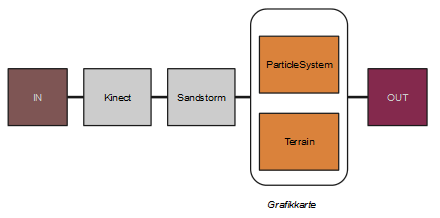
\includegraphics[width=0.6\textwidth]{graphics/flow.png}
	\caption{Datenfluss}
	\label{fig:dataFlow}
\end{figure}

\section{Die Modularisierung}
Um eine parallele Entwicklung und spätere Erweiterbarkeit sicherzustellen soll modulbasiert entwickelt werden. Das Projekt lässt sich in drei Kategorien gliedern. Bestandteile sind das ParticleSystem (ParticleSystem), die Kinect Ansteuerung (SandstormKinect) und einen Controller (Sandstorm), welcher Events entgegen nimmt und für die Verarbeitung zuständig ist. Die Basis bildet die DrawableGameCompontent, welches jeder Komponente einen eigenen Kontext zuweist. Dies bedeutet das jede DrawableGameCompontent ein separates Projekt darstellt und unabhängig betrieben werden kann. Die Strukturierung ist in Abbildung \ref{fig:component} dargestellt.

\begin{figure}[h!]
	\centering
	\vspace*{20px}
	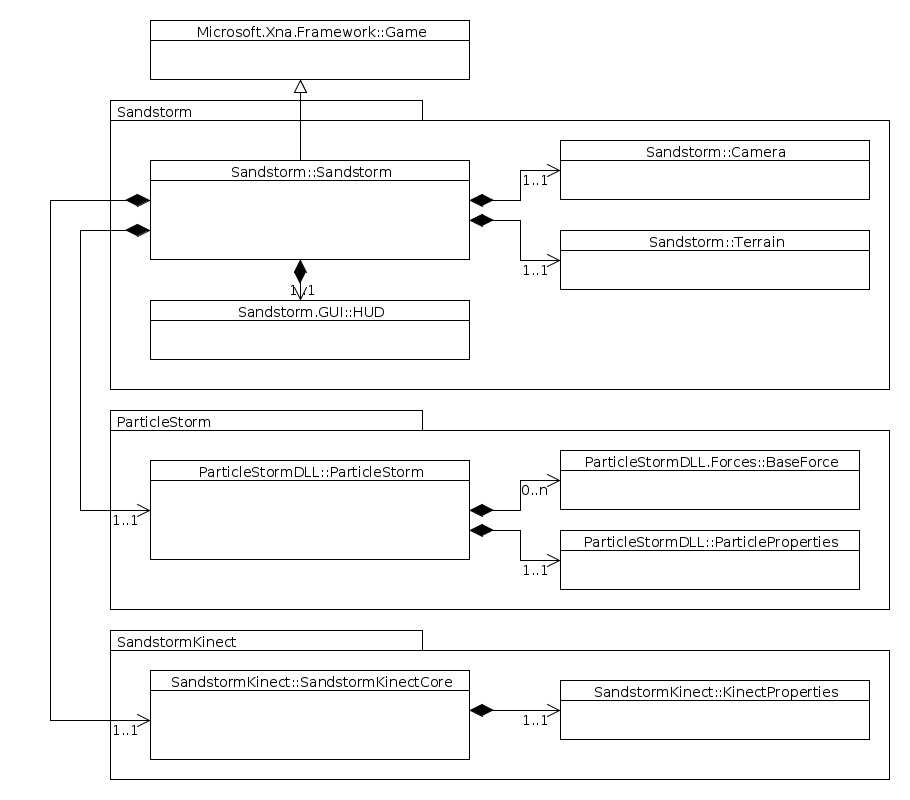
\includegraphics[width=0.99\textwidth]{graphics/overview.png}
	\caption{Kompontenten}
	\label{fig:component}
\end{figure}

\section{Die Component Properties} \label{PropSec}
Um das  System so dynamisch wie möglich zu gestalten, sollen Sammelcontainer für Systemparameter eingeführt werden, sogenannte Properties.
Diese Properties sind vergleichbar mit Konfigurationsdateien. Ändert man einen Wert innerhalb einer Properties so wird der neue Wert sofort vom restlichen System übernommen. Für jede Kategorie (Physikengine,RenderEngine,Kinect..) soll ein solcher Container genutzt werden, um für verschiedene Anwendungsszenarien Default-Wert zu hinterlegen und diese bei Bedarf zu laden oder zu speichern. Zusätzlich ermöglichen diese, die Erzeugung eines komplett dynamischen User Interface (s. Abschnitt \ref{GUISec}).

\end{Spacing}
\newpage
\clearpage
%% End Of Doc

%\clearpage
% !TEX root = ../report.tex
\chapter{Grundlagen}
\begin{Spacing}{\mylinespace}

Nachfolgend werden die benötigten Grundlagen erläutert welche hilfreich sind, um dem
Inhalt und Designentscheidungen späterer Kapitel besser folgen zu können.
\end{Spacing}

% !TEX root = ../../report.tex
\begin{Spacing}{\mylinespace}
\section{CPU vs. GPU}
CPUs und GPUs weisen grundlegend verschiedene Architekturen auf.
\begin{figure}[h!]
	\vspace*{30px}
	\centering
	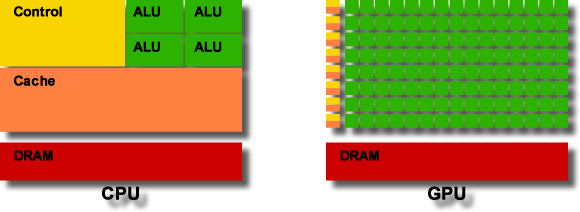
\includegraphics[width=320px]{graphics/GPUvsCPU.png}	
	\caption{CPU- vs. GPU-Architektur}
	\label{fig:GPUvsCPU}
\end{figure}

Während eine CPU einen relativ großen Befehlssatz hat um Ganz- oder Fließkommazahlen zu verarbeiten, besitzt hingegen eine GPU einen sehr kleinen Befehlsatz und kann lediglich Fließkommazahlen verarbeiten.
Der große Vorteil einer GPU jedoch ist das sie die Möglichkeit besitzt Berechnungsaufgaben an verschiedene kleinere CO-Prozessoren sogenannte Shader-Units abzugeben. Durch das zuweisen einer Aufgabe pro Shader-Unit erlaubt eine GPU somit das hoch-parallele abarbeiten von Aufgaben - solange diese unabhängig voneinander sind.
Diese parallele Programmierung hat jedoch auch Nachteile.
Nicht nur das es einer speziellen Programmierung benötigt - sogenannte Shader-Programmierung (Shader-Programme).
Sondern es setzt auch Vorraus, das jede Shader-Unit das gleiche Shader-Programm ausführt. Besitzen jedoch die zu verarbeitenden Berechnungen genug Unabhänigkeit, so kann eine erhebliche Beschleunigung durch den Einsatz einer GPU welche meist hunderte von Shader-Units besitzt, erzielt werden.


\section{GPU-Programmierung}

Die GPU-Programmierung unterscheidet sich in vielen Punkten von der CPU-Programmierung. Für ein besseres Verständnis ist es von Vorteil, wenn man die einzelnen Arbeitsschritte einer GPU, von der Eingabe bis zur Ausgabe kennt. Diese wollen wir folgend, mit Hilfe eines kleinen Beispiels erläutern.

\begin{figure}[h!]
	\vspace*{20px}
	\centering
	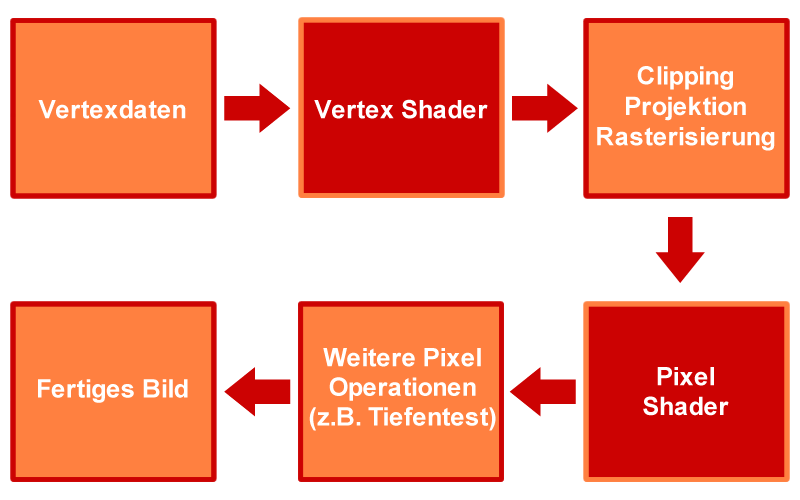
\includegraphics[width=330px]{graphics/pipeline.png}	
	\caption{Die GPU Pipeline}
	\label{fig:pipeline}
\end{figure}

Abbildung \ref{fig:pipeline} zeigt die einzelnen Arbeitsschritte einer GPU. Starten wir, mit unserem Beispiel im ersten Schritt \textit{Vertexdaten}. Um das Beispiel möglichst simple zu gestalten, wollen wir ein einfaches rotes Rechteck generieren und ausgeben. Dazu muss man wissen, das eine GPU immer nur einzelne Punkte oder Dreiecke zeichnen kann. Um unser Rechteck zu erzeugen benötigen wir also zwei Dreiecke, die jeweils aus drei Punkten bestehen. (s. Abbildung \ref{fig:Viereck}.

\begin{figure}[h!]
	\vspace*{30px}
	\centering
	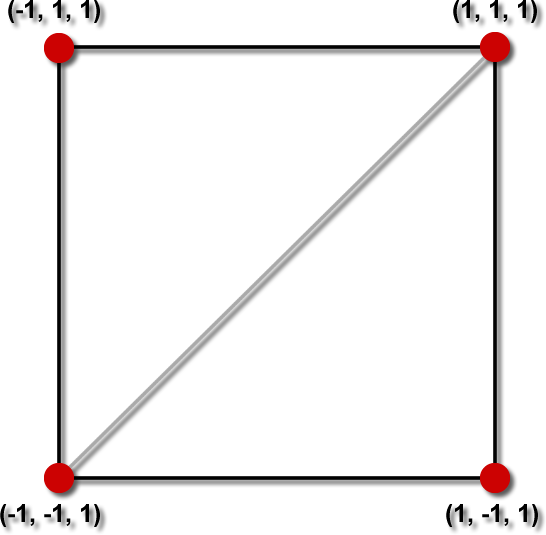
\includegraphics[height=130px]{graphics/Quad2.png}	
	\caption{Aufbau des Rechtecks}
	\label{fig:Viereck}
\end{figure}

\subsection{VertexBuffer}
Um die insgesamt sechs Punkte unseres Rechtecks an die GPU zu übergeben, erzeugen wir einen sogenannten \textit{Vertex Buffer}. Dieser stellt einen Speicherbereich, für unsere einzelnen Punkte, auf der GPU dar. Die Punkte werden in dem \textit{Vertex Buffer} so abgelegt, dass sie sequentiell abgearbeitet unsere beiden Dreiecke ergeben. Hierbei muss auch die Reihenfolge der Punkte pro Dreieck beachtet werden. Je nach Einstellung, kann diese im Uhrzeigersinn oder gegen den Uhrzeigersinn angegeben werden. Abbildung \ref{fig:VertexBuffer} zeigt den benötigten \textit{Vertex Buffer} zur Erzeugung der beiden Dreiecke im Uhrzeigersinn.

\begin{figure}[h!]
	\vspace*{15px}
	\centering
	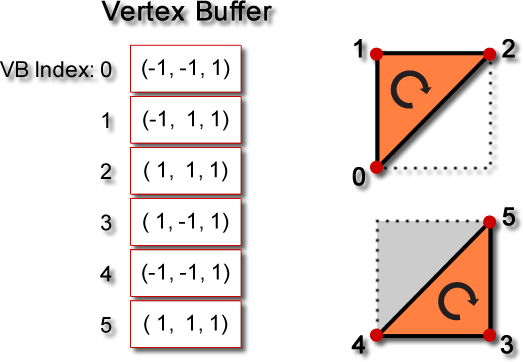
\includegraphics[height=120px]{graphics/vertexbuffer2.png}	
	\caption{Der VertexBuffer unseres Rechtecks}
	\label{fig:VertexBuffer}
\end{figure}

\subsection{IndexBuffer}
Wie man in Abbildung \ref{fig:VertexBuffer} erkennen kann, enthält unser erzeugter \textit{Vertex Buffer} duplizierte Einträge an den Stellen (0-4) und (2-5). Bei dem in unserem Beispiel verwendeten Rechteck, fällt dieser unnötige Speicherverbrauch nicht großartig ins Gewicht. Bei weitaus komplexeren Modellen, können diese doppelten Einträge jedoch schnell zu einem Problem werden. Um doppelte Einräge im \textit{Vertex Buffer} zu verhindern, werden sogenannte \textit{Index Buffer} eingesetzt. Diese enthalten Indizes die auf die einzelnen Einträge im \textit{Vertex Buffer} referenzieren. Abbildung \ref{fig:IndexBuffer} zeigt, den für unser Beispiel benötigen, Index- und Vertex Buffer. Wie man sieht sind die doppelten Einträge aus unserem \textit{Vertex Buffer} verschwunden und die Reihenfolge zum Zeichen der beiden Dreiecke, wird nun durch den \textit{Index Buffer} vorgegeben. 
 

\begin{figure}[h!]
	\vspace*{15px}
	\centering
	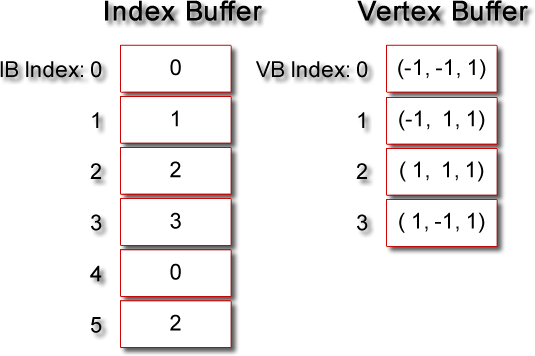
\includegraphics[height=120px]{graphics/indexbuffer2.png}	
	\caption{Der Vertex- und Index Buffer unseres Rechtecks}
	\label{fig:IndexBuffer}
\end{figure}

\subsection{Vertex Shader}
Nachdem wir unsere Daten nun erfolgreich auf die GPU übertragen haben, geht es weiter mit dem nächsten Schritt, dem \textit{Vertex Shader}. Shader sind die programmierbaren Einheiten einer GPU, in denen wir selbst Einfluss auf die Grafikpipeline nehmen können. Dazu zählen, der \textit{Vertex Shader}, auf den wir hier einen Blick werfen werden, der \textit{Pixel Shader}, den wir uns danach betrachten und bei neueren GPU's der \textit{Geometry Shader}, den wir hier nicht behandeln werden.
\\\\
Der \textit{Vertex Shader} arbeitet auf der \textit{Vertex}-Ebene, das sind unsere einzelnen Punkte. Diese können hier noch einmal manipuliert oder transformiert werden.
Der Quellcode \ref{vertexshader} zeigt einen minimalen \textit{Vertex Shader}. Dieser bekommt unsere Punkte übergeben, transformiert diese mit der Matrix \textit{worldViewProj} vom \textit{Objectspace} in den \textit{Screenspace} und gibt die transformierten Punkte an den nächsten Schritt der Pipeline weiter.

\begin{lstlisting}[captionpos=b, caption=Vertex Shader unseres Rechtecks., label=vertexshader]
01 float4x4 worldViewProj;
02
03 float4 vertexshader(float4 position)
04 {
05   return mul(position, worldViewProj);		
06 }
\end{lstlisting}

\subsection{Clipping, Projektion, Rasterisierung}
In diesem Schritt werden unsere in den \textit{Screenspace} transformierten Punkte auf einzelne Bildschirmpixel abgebildet (Rasterisierung) und alle überflüssigen Pixel, die außerhalb des Bildschirmbereichs liegen, verworfen (Clipping).

\subsection{Pixel Shader}
Nachdem unsere dreidimensionalen Punkte, im vorherigen Schritt zu zweidimensionalen Bildschirmpixel gerastert wurden, kommen wir nun zur nächsten programmierbaren Einheit einer GPU, dem \textit{Pixel Shader}. Dieser arbeitet auf textit{Pixel}-Ebene und ist für die Einfärbung zuständig. Der Quellcode \ref{pixelshader} zeigt einen minimalen \textit{Pixel Shader}. Dieser färbt alle Pixel unseres Rechtecks rot ein.

\begin{lstlisting}[captionpos=b, caption=Fragment Shader unseres Rechtecks., label=pixelshader]
01 float4 pixelshader()
02 {
03   return float4(0.8, 0.0, 0.0, 1.0);
04 }
\end{lstlisting}

\subsection{Weitere Pixel Operationen}
Auf die weiteren Pixel Operationen wie den Tiefentest, der für die Tiefensortierung der einzelnen Pixel zuständig ist, wollen wir der Einfachheit unseres Beispiels hier nicht näher eingehen.

\subsection{Fertiges Bild}
Als Resultat unseres kleinen Beispiels, erhalten wir am Ende, das in Abbildung \ref{fig:exampleRes} gezeigte, rot gefärbte Rechteck.

\begin{figure}[h!]
	\vspace*{15px}
	\centering
	
\includegraphics[height=120px]{graphics/exampleRes.png}	
	\caption{Der Ergebnis unseres kleinen Beispiels.}
	\label{fig:exampleRes}
\end{figure}

\end{Spacing}
\clearpage
%% End Of Doc
%% !TEX root = ../../report.tex

\section{Mathematische Verfahren}

\subsection{Verzerrung von Bildern}

\subsection{Blending}
Blending ist ein Verfahren welches es ermöglicht überlappende Teilbereiche von zwei Objekten zu definieren.
Hierbei spielt der Alpha-Kanal eine große Rolle, dieser besagt wie durchsichtig ein Objekt ist und somit die Dominanz beim mischen von Farben. Es gibt verschiedene Ausprägungen des Blendings, im einfachsten Fall - so wie auch in unserem Projekt, kommt das additive Alpha-Blending zum Einsatz. Besitzt der Alpha Wert einen hohen Wert (nahe 1) so ist das Objekt sehr dominant und kaum bis garnicht durchsichtig. Ist der Alpha Wert hingegen niedrig (nahe 0) so ist das Objekt durchsichtig vergleiche hierzug Abbildung \ref{fig:AlphaBlending}.
\begin{figure}[h!]
	\centering
	\vspace*{30px}
	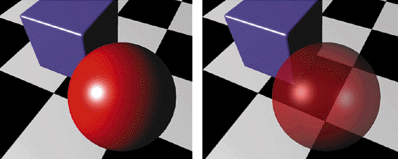
\includegraphics[width=320px]{graphics/blending.png}	
	\caption{Additives Alpha-Blending\protect\footnotemark}
	\label{fig:AlphaBlending}
\end{figure}
\footnotetext{Quelle: \url{http://common.ziffdavisinternet.com/encyclopedia_images/_ALPHACH.GIF}}

\subsection{Billboarding}
Um unsere Vorgabe der Echtzeitfähigkeit zu erfüllen benötigt es ein paar Tricks, die es erlauben die Komplexität unseres Renderers zu minimieren, gleichzeitig jedoch darf der Zuschauer diese Manipulation nicht bemerken.
Eine beliebte Technik hierfür ist das Billboarding. Die Idee des Billboardings basiert darauf, komplexe geometrische 3D-Objekte auf ein zweidimensionales Rechteck das sogenannte Billboard runterzubrechen. 
Bei dem Billboard handelt es sich meist um ein vorher berechnetes Bild von dem ursprünglich darzustellenden 3D-Objekts.
Anschließend wird dieses Billboard zur Kamera ausgerichtet. Durch den zusätzlichen Einsatz von Blending überlappen diese 2D Objekte Objekte dann und erzeugen somit einen 3D-Effekt. Dem Zuschauer fällt es somit sehr schwer zu erkennen, das es sich bei dem gezeigten Objekt um eine zweidimensionale Kopie des 3D-Objektes handelt.
Diese Technik wird hauptsächlich dazu verwendet die benötigten Rechenoperationen für Objekte welche in der Ferne liegen zu minimieren. 
Kommt die Kamera dem tatsächlichen Objekten sehr nahe, wird meist mittels einer Interpolation zwischen dem Billboard und dem tatsächlichen 3D-Objekt umgeschaltet.
\end{Spacing}
\newpage
\clearpage
%% End Of Doc

\clearpage
%% End Of Doc
\clearpage
% !TEX root = ../report.tex
\chapter{Realisierung}
\begin{Spacing}{\mylinespace}

In diesem Kapitel wird die Realisierung des Projekts erläutert. Begonnen mit dem Hardwareaufbau über die Wahl der Frameworks, das Grundgerüst der Anwendung, die Integration der \textit{Kinect}-Kamera, dem Aufbau des Kamera-Systems und der Terrain-Darstellung bis zum Partikelsystem samt Physik.  \\

% !TEX root = ../../report.tex
\section{Hardwareaufbau}
\begin{Spacing}{\mylinespace}

Die Hardware \\

Beschreibung wie der Tisch gebaut ist\\

\begin{figure}[hbtp]
	\centering
	\label{fig:laboraufbauaufbau}
	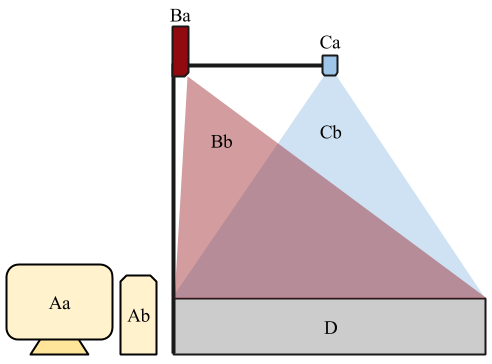
\includegraphics[width=0.8\textwidth]{graphics/Aufbau.png}
	\caption{Laboraufbau}
\end{figure}

\begin{enumerate}  
      \item (A) Steuerrechner
      \begin{enumerate}
         \item Kontrollbildschirm
         \item Rechner
      \end{enumerate}
      \item (B) Projektion
      \begin{enumerate}
         \item Projektor
         \item Projektionsperspektive
      \end{enumerate}
      \item (C) Höhenerfassung
      \begin{enumerate}
         \item Microsoft Kinect
         \item Erfassungsperspektive
      \end{enumerate}
      \item (D) Sandkasten
 \end{enumerate}
   
Was für Rechner dranne hängt\\
Was für Beamer dranne hängt\\
Was das mit dem Sand war\\

\begin{figure}[hbtp]
	\centering
	%Bild oben
	\subbottom[Kinect Hardware]{
	\label{fig:kinHW}
	\inputTikZ{graphics/kinectHW}
	}
	\hfill
	% Bild unten
	\subbottom[Kinect Sichtfeld im Nahmodus]{
	\label{fig:fov}
	\inputTikZ{graphics/fov}
	}
	\caption{Kinect Sensor}
\end{figure}

Die Konstruktion\\
Der Aufbau

\end{Spacing}
\newpage
\clearpage
%% End Of Doc
\clearpage
% !TEX root = ../report.tex
\section{Die Frameworks}
\begin{Spacing}{\mylinespace}

\begin{figure}[h!]
	\centering
	\includegraphics[width=300px]{graphics/xna.png}
\end{figure}

Für die Interaktion mit der \textit{Kinect}-Kamera und der Darstellung der Landschaft und des Partikelsystems haben wir uns für das \textit{XNA Game Studio 4.0} und das Kinect SDK von \textit{Microsoft} entschieden. Das \textit{XNA Game Studio} ist eine Programmierumgebung die auf \textit{Visual Studio} basiert und zur Entwicklung von Spielen für \textit{Windows-Phone}, \textit{XBox 360} und \textit{Windows}-basierten Computern entworfen wurde. Bestandteil des \textit{XNA Game Studio} ist das \textit{XNA Framework}, welches mehrere auf dem \textit{.Net-Framwork} basierende Bibliotheken vereint und eine sehr einfache und angenehme Schnittstelle zu diesen bereitstellt.
\\\\
Dazu gehören:

\begin{description}
	\item[DirectX] \hfill \\
	DirectX ist eine API für hochperformante Multimedia-Anwendungen und kommt meist bei der Hardware-beschleunigten Darstellung von 2D- und 3D-Grafiken zum Einsatz. 
	\item[XInput] \hfill \\
	XInput ist eine API zur Verarbeitung von Benutzereingaben über Maus, Tastatur und den \textit{XBox 360} Kontroller.
	\item[XACT] \hfill \\
	XACT(Microsoft Cross-Platform Audio Creation Tool) stellt einfache Schnittstellen zur Audiowiedergabe und der Verknüpfung von Sounds an bestimmte Ereignissen bereit.
\end{description}

In unserer Implementierung wird ausschließlich DirectX für die Darstellung und XInput für die Verarbeitung der Benutzereingaben genutzt. Zudem kommt zusätzlich das \textit{Kinect SDK} zur Ansteuerung der \textit{Kinect}-Kamera zum Einsatz, welches auch auf dem \textit{.Net-Framework} basiert und sich dadurch nahtlos und ohne weitere Anpassungen in das System integrieren lässt.

\end{Spacing}
\newpage
\clearpage
%% End Of Doc
\clearpage
%\input{include/realisierung/renderer}
%\clearpage
% !TEX root = ../../report.tex
\section{Kinect}
\begin{Spacing}{\mylinespace}

\subsection{Aufbau und Funktion}

Die Kinect ist als eigenständige Bibliothek konzipiert und kann so in beliebige Projekte integriert werden. Das interne Vorgehen ist in Abbildung \ref{fig:kinectdll} schematisch dargestellt. 

\begin{figure}[hbtp]
	\vspace{15px}
	\centering
	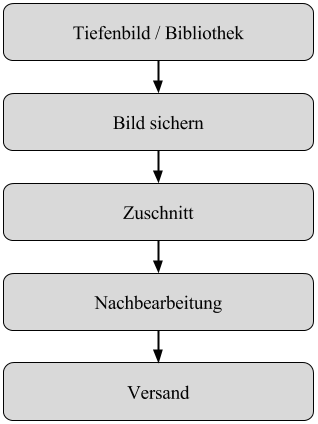
\includegraphics[width=0.4\textwidth]{graphics/block_dll.png}
	\caption{Laboraufbau}
	\label{fig:kinectdll}
\end{figure}

Nach dem Einbinden des Kinekt SDK kann sich ein Objekt der Kinect der Kinect erstellt sowie parametrisiert werden. Diese Objekt bietet nun die Möglichkeit sich auf einen Eventhandler zu registrieren, welcher die Auslieferung der Daten von Seitens der Kinect übernimmt. Dies wird alle in einem separaten Thread ausgeführt um die Leistung des Systems so optimal wie möglich zu halten.

Wird ein Bild empfangen wird, muss es als erstes in einer eigenen Struktur gesichert werden. Anschließend wird es auf die Zielauflösung zugeschnitten.
Dies ist nötig da der Sandkasten eine quadratische Form hat, das Bild jedoch im Format 3:4 (Auflösung von 640x480 Bildpunkte) von der Kinect kommt.
Als nächste Schritt muss der Bildaufbau verändert werden das das Bild um 180 Grad gedreht abgenommen wird. Dies hängt mit dem Hardwareaufbau zusammen, worin die Kinect befestigt ist. Weiterhin müssen die Tiefenwerte angepasst und auf die höhe des Sandkastens normiert werden. Der Grund hierfür liegt in der späteren Darstellung. Um die Farben der Höhenlinien angenehm verteilt anzeigen zu lassen, ist ein breites Spektrum an Tiefendaten erforderlich. Alle Bilddaten welche nicht im gewünschten Bereich des Sandkastens liegen werden auf unendlich gesetzt.

Abschließend werden die aufbereiteten Daten als Array mit einem Event verschickt und es kann ein weiteres Tiefenbild folgen. Für das Versenden wird deine eigene EventArgument-Klasse verwendet um eine spätere Erweiterung, z.B. hinzufügen von Metadaten, zu erleichtern.

\subsection{Nutzung}

Die Einbindung der Bibliothek ist über einen Verweis zu realisieren. Wenn die erfolgreich geschehen ist kann ein neues Objekt vom Typ "SandstormKinectCore" erstellt werden. Dieses Objekt bietet dann die Registrierung auf einen EventHandler an, welches genutzt werden soll.
Über die öffentlichen Methoden "StartKinect" sowie "StopKinect" kann nun der Betrieb hergestellt werden. Bei jedem neuen Tiefenbild wird über das Event ein Aufbereitetes Tiefenbild versand und kann weiter verwendet werden.

\end{Spacing}
\newpage
\clearpage
%% End Of Doc
\clearpage
% !TEX root = ../../report.tex
\section{Das Terrain}
\begin{Spacing}{\mylinespace}

Nachdem das Grundgerüst der Anwendung stand und wir die Kinect Kamera erfolgreich eingebunden hatten ging es daran uns um die Umsetzung der Terraindarstellung zu kümmern.

\subsection{Die Grundgeometrie}
Als Grundgeometrie für die Darstellung unseres Terrains erzeugen wir ein flaches reguläres Gitter, dass in der X-Z-Ebene aufgespannt ist (s. Abbildung \ref{fig:grid}). Die Größe und die Anzahl der Unterteilungen des Gitters wurde variabel gestaltet, um im späteren Verlauf der Entwicklung, einfacher unterschiedliche Konfiguration zu testen. 

\begin{figure}[h!]
	\centering
	\vspace*{10px}
	\includegraphics[width=0.6\textwidth]{graphics/grid.png}
	\caption{Reguläres Gitter des Terrains.}
	\label{fig:grid}
\end{figure}

\subsection{Die Höhendaten}
Um mit dem zuvor erstellten regulären Gitter ein vollständiges Abbild unserer Sandkastenlandschaft zu repräsentieren, musste nun noch ein Weg gefunden werden die von der Kinect gelieferten Höhendaten in das Model zu integrieren. Abbildung \ref{fig:resize} zeigt die erhaltenen Daten der Kinect.
\\
\begin{figure}[h!]
	\centering
	\includegraphics[width=0.6\textwidth]{graphics/resize.png}
	\caption{Die gelieferten Daten.}
	\label{fig:resize}
\end{figure}  

Um die vorarbeitenden Daten nun auf das reguläre Gitter zu übertragen, kamen zwei unterschiedliche Ansätze in Frage:
\begin{description}
	\item[1. Mit Hilfe der CPU] \hfill \\
	Beim ersten Ansatz werden die Daten direkt auf der CPU verarbeitet und in das reguläre Gitter integriert. Ein großer Nachteil dieses Ansatzes ist allerdings, dass bei jeder Aktualisierung der sogenannte \textit{VertexBuffer}, mit dessen Hilfe die Geometriedaten an die GPU übertragen werden, komplett neu aufgebaut werden muss. Dieser Vorgang ist sehr kostenintensiv und würde die Echtzeitfähigkeit unserer Anwendung stark einschränken.
	\item[2. Mit Hilfe der GPU] \hfill \\
	Beim zweiten Ansatz kann dieser kostenintensive Neuaufbau des Vertexbuffers durch moderne Shader-basierte Verfahren umgangen werden. Dazu wird aus den Daten eine Textur (Heightmap s. Abbildung \ref{fig:heightmap}) erzeugt und anschließend mit den Geometriedaten des regulären Gitters zusammen an die GPU übertragen. Im Vertex-Shader kann jetzt mit Hilfe des \textit{Vertex Texture Fetch} (VTF) Verfahrens direkt auf diese Textur und die enthaltenen Höhendaten zugegriffen und für die Manipulation der Y-Position der einzelnen Vertizes genutzt werden.
\end{description}

Entschieden haben wir uns letztendlich für den zweiten Ansatz, da er das weitaus höhere Potenzial zur Echtzeitfähigkeit bietet, welche für unsere Anwendung eine sehr wichtige Rolle spielt und darüber hinaus auch ressourcensparender ist. 

\begin{figure}[h!]
	\centering
	\vspace*{20px}
	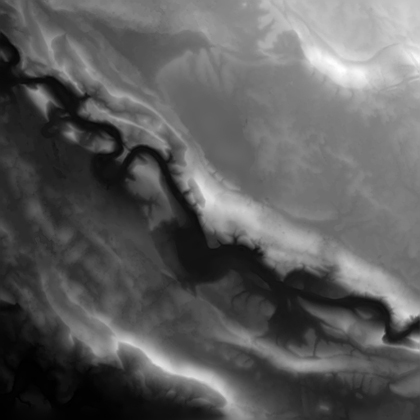
\includegraphics[width=200px]{graphics/heightmap.jpg}
	\caption{In einer Textur abgelegte Höhendaten (Heightmap).}
	\label{fig:heightmap}
\end{figure}

\subsection{Die Darstellung}
Nachdem nun die Grundgeometrie erzeugt, die Höhendaten vor verarbeitet an die GPU übertragen und die Y-Position der Vertices manipuliert wurden, können wir nun unser Terrain endlich darstellen. Einheitlich eingefärbt, bekommen wir allerdings ein Ergebnis dass nicht wirklich an eine Landschaft erinnert (s. Abbildung \ref{fig:singleColors}). 

\begin{figure}[h!]
	\centering
	\vspace*{20px}
	\includegraphics[width=320px]{graphics/singleColor.png}
	\caption{Darstellung mit nur einer Farbe.}
	\label{fig:singleColors}
\end{figure}

Dieses Erscheinungsbild lässt sich durch ein fehlendes Beleuchtungssystem und die dadurch fehlende Schattierung der Szene erklären. Da die Implementierung eines kompletten Beleuchtungssystems für unsere Anwendung allerdings wenig Sinn machen würde, lösen wir das oben gezeigte Darstellungsproblem mit Hilfe von verschiedenen Farben für die unterschiedlichen Höhenwerte. Die einfachste Umsetzung dafür wäre direkt die Farbwerte aus der Höhentextur zu nutzen, wodurch ein Graustufenverlauf von dunkel (niedrig) zu hell (hoch) entstehen würde (s. Abbildung \ref{fig:differentColors}a). Hierdurch erhalten wir zwar eine korrekte Darstellung unseres Terrains, jedoch sind Graustufen mehr als ungeeignet für die spätere Projektion auf den Sand. Aus diesem Grund haben wir eine Möglichkeit zur benutzerdefinierten Wahl des Farbverlaufs implementiert. Diese besteht aus vier frei wählbaren Farben für vier unterschiedliche Höhenbereiche welche im Shader linear interpoliert werden (s. Abbildung \ref{fig:differentColors}b,c).    

\begin{figure}[h!]
	\centering
	\vspace*{30px}
	\includegraphics[width=\textwidth]{graphics/differentColors.png}
	\caption{(a) Einfärbung anhand der Höhentextur. (b, c) Einfärbung anhand eines benutzerdefinierten Farbverlaufs.}
	\label{fig:differentColors}
\end{figure}

Um die Höhenunterschiede bei der Projektion auf den Sand noch deutlicher erkennbar zu machen, haben wir am Ende des ersten Projektsemesters noch mit der Darstellung von Höhenlinien experimentiert und im laufe des zweiten Projektsemester letztendlich vollständig integriert.

Die erste experimentelle Version (s. Abbildung \ref{fig:contourLines}a) arbeitete ausschließlich auf den reinen Höhendaten an einem einzelnen Punkt, weshalb an manchen Stellen noch sehr großflächige, schwarze Bereiche auftraten. Bei der endgültigen Version (s. Abbildung \ref{fig:contourLines}b) flossen schließlich noch zusätzliche Informationen aus den Nachbarbereichen mit in die Berechnung ein, um eine einheitliche Stärke der Höhenlinien zu gewährleisten und größere, schwarze Bereiche auszuschließen.  


\begin{figure}[h!]
	\centering
	\vspace*{50px}
	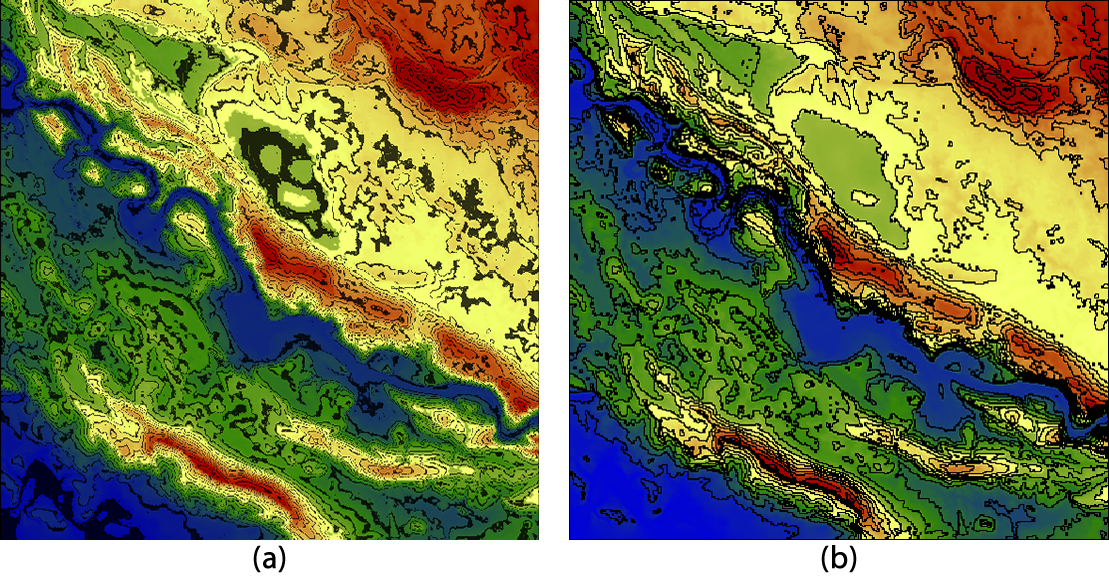
\includegraphics[width=400px]{graphics/contourLines2.png}
	\caption{(a) 1. experimentelle und (b) endgültige Darstellung der Höhenlinien.}
	\label{fig:contourLines}
\end{figure}


\end{Spacing}
\newpage
\clearpage
%% End Of Doc
\clearpage
% !TEX root = ../report.tex
\section{Das Kamerasystem}
\begin{Spacing}{\mylinespace}

Um eine Navigation in unserer 3D Szene, sowie eine einfache Art der Kalibrierung zu ermöglichen, wurde ein kleines, erweiterbares Kamerasystem entwickelt. Das System besteht aus zwei Hauptkomponenten, der Kamera-Klasse und der Kamerakontroller-Klasse.

\begin{description}
	\item[Kamera] \hfill \\
	Die Kamera-Klasse stellt alle Grundfunktionen einer virtuellen Kamera zur Verfügung. Dazu gehören neben der Translation und der Rotation auch unterschiedliche Arten der Projektion (Perspektivisch, Orthografisch) und verschiedene Kamera-Modi (Orbital, Walk, Fly) zur Navigation. \\\\
	Um den sogenannten \textit{Gimbal Lock} zu vermeiden, welcher bei der Verwendung von \textit{Eulerwinkeln} zur Rotation entstehen kann und in speziellen Fällen den Verlust eines kompletten Freiheitsgrades bewirkt, setzten wir in unserem System auf den Einsatz von \textit{Quantenionen} zur Rotation der Kamera. Diese bieten neben der Vermeidung des \textit{Gimbal Locks} auch eine weitaus effizientere Berechnung der Transformationen.   
	\begin{figure}[h!]
	\centering
	\vspace*{10px}
	\includegraphics[width=160px]{graphics/cam.png}
	\caption{Grundfunktionen der Kamera.}
	\label{fig:cam}
	\end{figure}
	\item[Kameracontroller] \hfill \\
	Die Kameracontroller-Klasse dient als Schnittstelle zwischen der Peripherie und der eigentlichen Kamera und ermöglicht somit eine saubere Trennung zwischen der Verarbeitung von Benutzereingaben und der eigentlichen Funktionalität der Kamera. Abbildung \ref{fig:Camerasystem} zeigt den groben Aufbau des Kamerasystems. 
	\begin{figure}[h!]
	\centering
	\vspace*{30px}
	\includegraphics[width=300px]{graphics/camcon.png}
	\caption{Aufbau des Kamerasystems.}
	\label{fig:Camerasystem}
	\end{figure}
\end{description}


\end{Spacing}
\newpage
\clearpage
%% End Of Doc
\clearpage
% !TEX root = ../report.tex
\section{Das Partikelsystem}
\begin{Spacing}{\mylinespace}

Nachdem wir im ersten Projektsemester mit unserem CPU-basierten Partikelsystem sehr schnell an die Grenzen des machbaren gestoßen waren, haben wir uns im zweiten Projektsemester kurzfristig dafür entschieden, das System noch einmal komplett zu überarbeiten und dieses Mal auf eine reine GPU Implementierung zu setzen.

\subsection{Die Anforderungen}

Als Anforderungen haben wir uns gesetzt, ein hoch flexibles und vom restlichen System getrenntes Partikelsystem zu entwickeln, welches die Fähigkeit bietet mehrere hunderttausend oder sogar Millionen von Partikeln in Echtzeit darzustellen.  

\subsection{Die Umsetzung}

Um unser angestrebtes Ziel zu erreichen, haben wir auf eine Kombination aus verschiedenen Techniken gesetzt, die wir folgend etwas genauer Beschreiben werden.
 
\begin{description}
	\item[Billboarding] \hfill \\
	Für die Darstellung unserer Partikel haben wir zwei unterschiedliche Techniken in Betracht gezogen. Bei der erste und einfacheren Technik wird ein Partikel durch einen einzelnen Vertex repräsentiert und anschließend, als farbiger Punkt, auf den Bildschirm gezeichnet. Da wir aber nicht auf die Möglichkeit verzichten wollten, bei Bedarf unseren Partikeln auch eine Textur zuzuweisen, haben wir uns für die zweite, etwas aufwendigere, Technik das \textit{Billboarding} entschieden.
\\\\
\textit{Billboards} bestehen aus zwei dreieckigen Polygonen die ein Rechteck bilden (s. Abbildung \ref{fig:BBQuad}).	Dieses Rechteck wird anschließend im Vertexshader, mit Hilfe der Viewmatrix der Kamera, so transformiert damit es immer in Richtung des Betrachters ausgerichtet ist. Durch diese Eigenschaft, lassen sich, mit sehr geringem Rechenaufwand, unterschiedlichste Effekte realisieren. In unserem Anwendungsfall, die Darstellung von Rauch beziehungsweise Nebel. 

\begin{figure}[h!]
	\centering
	\vspace*{30px}
	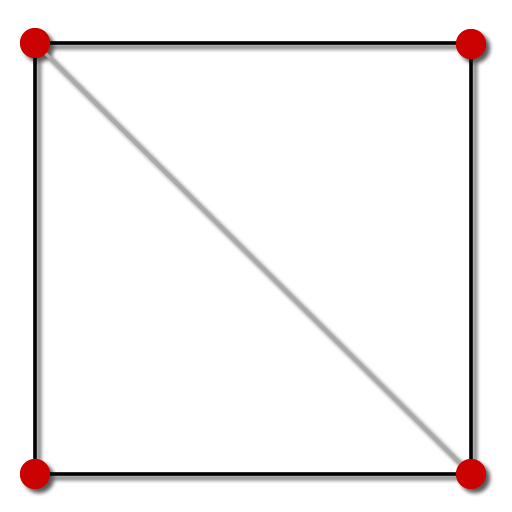
\includegraphics[width=110px]{graphics/billboardQuad.png}
	\caption{Aufbau des Rechtecks für ein Billboard.}
	\label{fig:BBQuad}
\end{figure}
\newpage
	\item[Instancing] \hfill \\
	Bei dieser Technik handelt es sich, um eine von der Grafikhardware bereitgestellten Funktionalität, zur Reduzierung von sogenannten \textit{Drawcalls}. Unter einem \textit{Drawcall} versteht man im Allgemeinen, das Zeichen eines Objekt mit einem bestimmten Material, einer Transformation und gegebenenfalls weiteren Eigenschaften. In unserem Fall wäre also jedes gezeichnete Partikel (Billboard) ein \textit{Drawcall}. Diese sind allerdings sehr teuer und bei der angestrebten Anzahl von über 1.000.000 Partikeln, wäre an eine Echtzeitfähigkeit nicht mehr zu denken gewesen. Somit entschieden wir uns für das \textit{Instancing}. Diese Technik erlaubt es 1.048.576 Instanzen der gleichen Geometrie, in unserem Fall die Billboards, in nur einem einzigen \textit{Drawcall} zu Zeichen. 
	
	\item[Rendertargets] \hfill \\
	In unserer vorherigen CPU-basierten Implementierung des Partikelsystems, war es ein leichtes, die benötigten Eigenschaften (Position, Geschwindigkeit, usw.) unserer Partikel, in einer dazu passenden Datenstruktur im RAM abzulegen und zu manipulieren. Bei der Neuimplementierung musste nun ein Weg gefunden werden, die Speicherung und Manipulation der Partikeleigenschaften, performant auf die GPU zu übertragen.
\\\\
Hierfür entschieden wir uns, für die Nutzung sogenannter \textit{Rendertargets}.   Diese repräsentieren eine spezielle Art von Texturen, für die neben dem standardmäßigen Lesezugriff auch Schreibzugriff zur Verfügung steht. Durch diese Eigenschaft, wird es möglich, \textit{Rendertargets} als Datencontainer zu nutzen und deren Inhalt direkt auf der GPU zu manipulieren.
\\\\
Zusätzlich zu den normalen \textit{Rendertargets}, unterstützt XNA auch \textit{Multiple Rendertargets}. Welche es ermöglichen, während eines Passes, in bis zu vier Rendertargets gleichzeitig zu schreiben. Mit dieser Technik war es uns nun möglich, unsere einzelnen Partikeleigenschaften in den einzelnen Farbkanälen der vier verfügbaren Rendertargets abzulegen (s. Abbildung \ref{fig:RTCahnnels}) und direkt auf der GPU zu manipulieren. 
	
\begin{figure}[h!]
	\centering
	\vspace*{55px}
	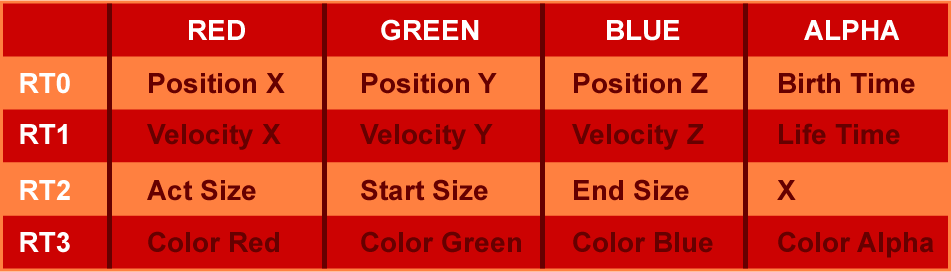
\includegraphics[width=410px]{graphics/RendertargetsChannels.png}
	\caption{Kanalbelegung der einzelnen Rendertargets.}
	\label{fig:RTCahnnels}
\end{figure}	

\newpage

	\item[Ping-Pong] \hfill \\
	Im Normalfall können \textit{Rendertargets}, innerhalb eines Passes, entweder nur gelesen oder nur geschrieben werden. Um diese Einschränkung zu umgehen und einen weiteren Pass einzusparen, setzten wir das sogenannte \textit{Ping-Pong} Verfahren ein. Bei diesem Verfahren, existiert von jedem \textit{Rendertarget} ein Duplikat (s. Abbildung \ref{fig:DoubleTarget}). Während eines Passes wird nun eines der Duplikate genutzt um Daten daraus zu lesen und das andere um die manipulierten Daten zurück zuschreiben. Im Anschluss an den Pass, werden die beiden \textit{Rendertargets} dann einfach ausgetauscht. Somit können im nächsten Pass, die zuvor geschrieben Daten gelesen werden und die alten Daten können überschrieben werden.
	
\begin{figure}[h!]
	\centering
	\vspace*{30px}
	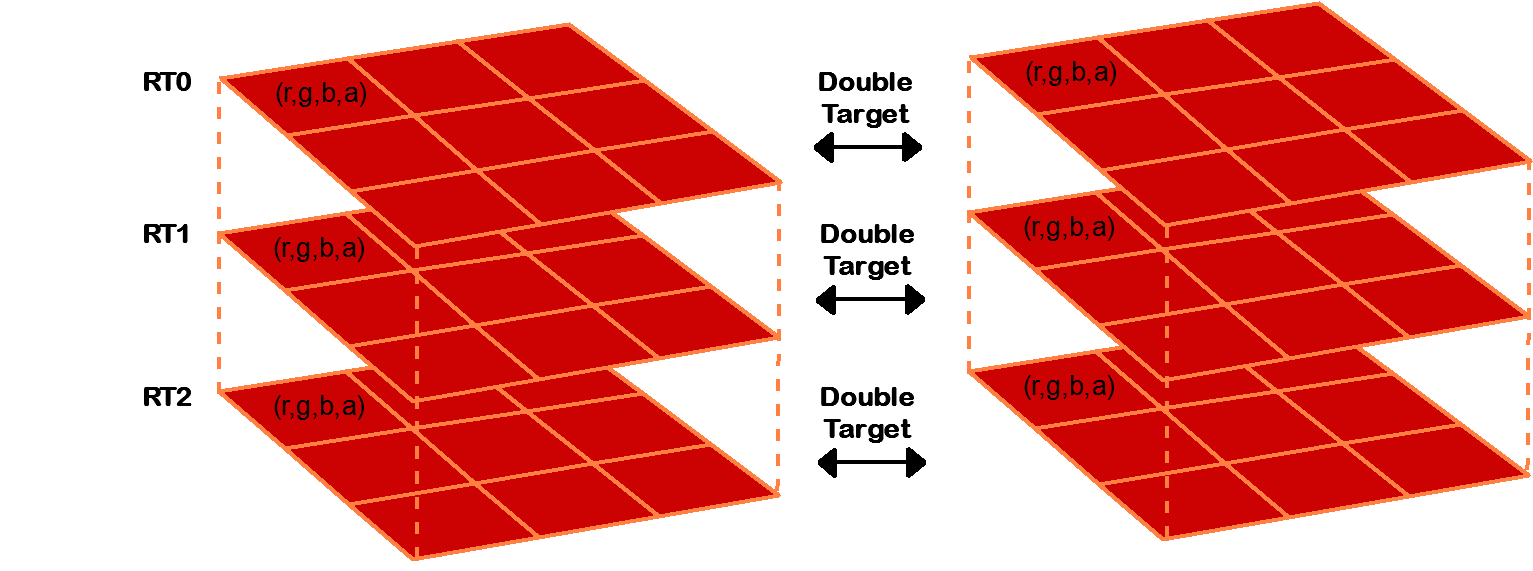
\includegraphics[width=350px]{graphics/DoubleTargets2.png}
	\caption{Duplizierte Rendertargets für Ping-Pong Verfahren.}
	\label{fig:DoubleTarget}
\end{figure}

	\item[Fullscreen-Pass/Offscreen-Pass] \hfill \\
Das Update unserer \textit{Rendertargets} und somit die Manipulation unserer Partikeleigenschaften, findet in einem sogenannten \textit{Fullscreen-Pass} statt, welcher vor dem eigentlichen Zeichen der \textit{Billboards} durchlaufen wird. Hierbei wird ein im \textit{Screenspace} positioniertes, Bildschirmfüllendes Rechteck genutzt, um ein 1-zu-1 Mapping des zu lesenden und des zu schreibenden \textit{Rendertargets} zu erreichen. Da dieser Pass keine Bildschirmausgabe zur folge hat, kann er auch als \textit{Offscreen-Pass} bezeichnet werden.

	\item[Blending] \hfill \\
Um bestimmte Effekte realistischer Darzustellen, bietet das neue Partikelsystem, optional die Möglichkeit, additives Blending (s. Abbildung \ref{fig:addBlending}) zu aktivieren. Dabei werden die Farben übereinanderliegender Partikel aufsummiert, wodurch Bereiche mit vielen übereinanderliegenden Partikeln heller erscheinen (s. Abbildung \ref{fig:particleResults}).

\begin{figure}[h!]
	\centering
	\vspace*{10px}
	
\includegraphics[width=100px]{graphics/additiveBlending.png}
	\caption{Additives Blending.}
	\label{fig:addBlending}
\end{figure}

\end{description}

\newpage
\subsection{Das Ergebnis}

Das Ergebnis unserer Neuimplementierung war mehr als zufriedenstellend. Am Ende hatten wir ein, vom restlichen System getrenntes und sehr flexibles Partikelsystem entwickelt, welches nun komplett auf der GPU lief und uns somit wieder mehr Ressourcen für andere Aufgaben, auf Seiten der CPU zur Verfügung standen. Auch unser, am Anfang noch für utopisch gehaltenes Ziel, eine Anzahl von über 1.000.000 Partikel in Echtzeit darzustellen, konnten wir mit dem neuen System erreichen. Bei über 1.000.000 Partikeln, läuft unsere Anwendung nun immer noch mit über 100 Frames die Sekunde, solche Ergebnisse konnten wir bei der vorherigen CPU-basierten Implementierung, selbst mit minimaler Anzahl an Partikeln nicht erreichen. Abbildung \ref{fig:particleResults} zeigt das Partikelsystem mit einigen unterschiedlichen Konfigurationen.

\begin{figure}[h!]
	\centering
	\vspace*{30px}
	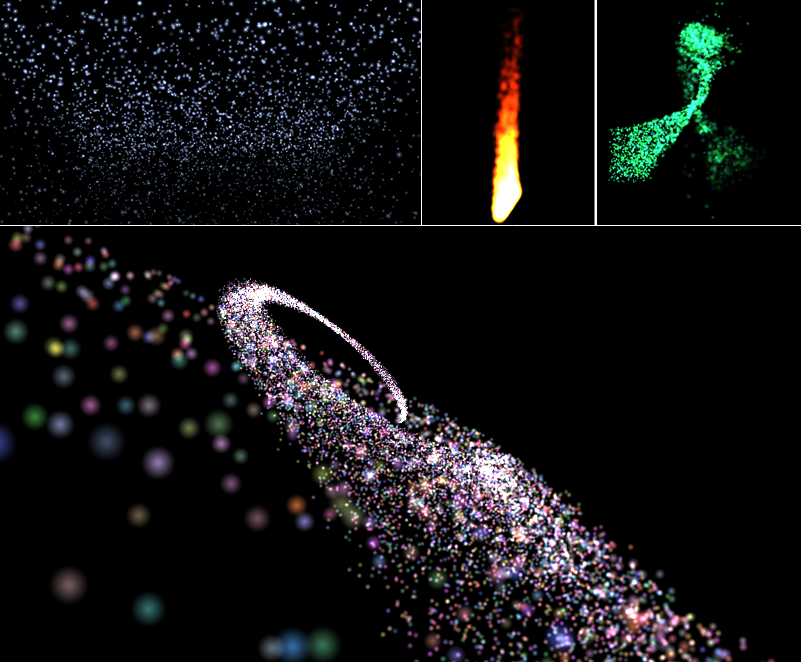
\includegraphics[width=410px]{graphics/ParticleResults.png}
	\caption{Partikelsystem mit unterschiedlichen Konfigurationen.}
	\label{fig:particleResults}
\end{figure}

\end{Spacing}
\newpage
\clearpage
%% End Of Doc
\clearpage
% !TEX root = ../report.tex
\section{Die Physik}
\begin{Spacing}{\mylinespace}
    Die Physik soll eine möglichst echtzeitfähige und
    realitätsgetreue Simulation von Luftströmung über eine dynamische Landschaft berechnen.
    Zu diesem Zweck sollten die Partikel des Partikelsystem die einzelnen
    Luftteilchen darstellen und mithilfe einer einfachen Physik
    die Interaktion zwischen diesen und ihrer Umgebung simuliert werden.
    \subsection{Komponenten}
        Jedes Luftpartikel besteht aus zwei dreidimensionalen Vektoren.
        Der Vektor $\vec{p}_{i}$ stellt dabei die Position des Partikels im
        Raum dar und der Vektor $\vec{v}_{i}$ beschreibt die aktuelle Bewegung des Partikels.
        Außerdem besitzen alle Partikel den gleichen Radius $r$ und einem
        Reibungskoeffizienten $\mu$, welcher bestimmt wie viel Energie ein Partikel
        bei einer Kollision verliert.
        Zusätzlich zu den Partikeln stehen Informationen über die Umgebung
        wie z.B. Höhendaten der Landschaft und verschiedene externe
        Kräfte ($F$), wie z.B. Gravitation, zur Verfügung.

        %\[ P_{i} = ( \vec{p}_{i}, \vec{v}_{i} ) , P_{i} \in P \]
        %\[ \vec{p}_{i} \in \mathbb{R}^{3} \]
        %\[ \vec{v}_{i} \in \mathbb{R}^{3} \]

        %\[ h_{xy} \in \mathbb{R} \]
        %\[ \vec{f}_i \in \mathbb{R}^{3} \]

    \subsection{Bewegung der Partikel}
        Um die Bewegung der Partikel zu simulieren wird in jeder Iteration,
        für jedes einzelne Partikel, der Bewegungsvektor $\vec{v}_{i}(t)$
        auf den Positionsvektor $ \vec{p}_{i}(t)$ aufaddiert.

        \[ \vec{p}_{i}(t+1) = \vec{p}_{i}(t) + \vec{v}_{i}(t) \]

        Auf diese Weise wird der Impuls solange erhalten bis der Bewegungsvektor
        durch Einwirkung äußerer Kräfte verändert wird.

        \begin{figure}[h!]
			\centering
			\vspace*{30px}
			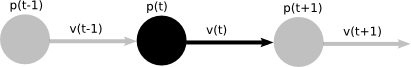
\includegraphics[width=0.7\textwidth]{graphics/Phys_bew0.png}
			\caption{Konstante Bewegung}
			\label{fig:BewegungPartikel}
		\end{figure}

		In diesem Fall wird angenommen das der zeitliche Abstand zwischen den
		einzelnen Iterationen konstant ist. Wenn die Dauer zwischen den Iterationen
		schwankt ist es ratsam dies zu kompensieren indem man den Bewegungsvektor
		$\vec{v}_{i}$ mit dem zeitlichen Abstand ($\Delta t$) zwischen den
		Iterationen multipliziert.
		 \[ \vec{p}_{i}(t+\Delta t) = \vec{p}_{i}(t) + \vec{v}_{i}(t) * \Delta t\]

    \subsection{Verrechnung externer Kräfte}
        In jeder Iteration wird die Wirkung externer Kräfte ($F$) auf das
        Partikel berechnet. Dabei wird jede der externen Kräfte ($\vec{f}_i$) auf den
        Bewegungsvektor $\vec{v}_{i}(t)$ aufaddiert.

        \[ \vec{v}_{i}(t+1) = \vec{v}_{i}(t) + \sum_{\vec{f}_{i} \in F}{\vec{f}_{i}} \]

		\begin{figure}[h!]
			\centering
			%\subfigure(1){ 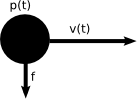
\includegraphics[width=0.2\textwidth]{graphics/Phys_bew1.png} \label{fig:ModForce1} }
			%\subfigure(2){ 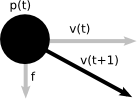
\includegraphics[width=0.2\textwidth]{graphics/Phys_bew2.png} \label{fig:ModForce2} }
			
\includegraphics[width=0.4\textwidth]{graphics/Phys_bew12.png}
			\caption{Bewegungsvektor vor(1) und nach(2) Modifikation durch eine externe Kraft }
			\label{fig:ModForce}
		\end{figure}

        Eine externe Kraft ist beispielsweise die Gravitation, welche die Partikel
        in die untere Richtung beschleunigt. Diese Wirkung kann dadurch erzielt
        werden indem beispielsweise der Vektor $( 0,-9.81,0 )$ zu der Menge der externen
        Kräfte hinzufügt wird.
		Diese schrittweise Aufaddierung führt, über mehrere Iteration hinweg gesehen,
		zur Beschleunigung des Partikels, wie es in der Abbildung \ref{fig:bewmod} dargestellt wird.
		\begin{figure}[h!]
			\centering
			\vspace*{30px}
			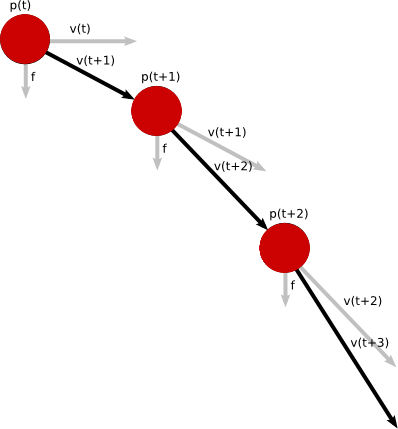
\includegraphics[width=0.7\textwidth]{graphics/Phys_bew3.png}
			\caption{Die auf das Partikel wirkende Kraft(f) bleibt konstant und
			die Bewegung wird bei jedem Rechenschritt weiter in die Richtung der
			Kraft beschleunigt}
			\label{fig:bewmod}
		\end{figure}

    \subsection{Kollisionserkennung von Partikeln mit der Umgebung}
    	Nachdem ein Partikel bewegt wurde, wird überprüft ob eine Kollision mit
    	der Heightmap vorliegt. Eine Kollision liegt vor wenn die vertikale Komponente
    	des Positionsvektors des Partikels einen niedrigeren Wert enthält als der
    	Höhenwert der Heightmap unterhalb der horizontalen Position des Partikels. Wenn dieser Fall
    	vorliegt befindet sich das Partikel unterhalb der Heightmap und ist
    	folglich während der letzten Positionsänderung in das Terrain eingedrungen
    	und es liegt nun eine Kollision vor.

    	Zusätzlich kann der Durchmesser des Partikels berücksichtigt werden
    	indem man den Radius zu dem Höhenwert der Heightmap aufaddiert und
    	dadurch eine Kollision erkannt wird bevor der Positionsvektor unterhalb
    	der tatsächlichen Heightmap liegt.

    \subsection{Kollisionsauflösung von Partikeln mit der Umgebung}
    	Wurde erkannt dass das Partikel mit der Heightmap kollidiert ist, wird eine
    	Kollisionsauflösung durchgeführt. Dabei wird zuerst die Flächennormale
    	der Heightmap ($\vec{n}$) an dem Ort der Kollision berechnet.

    	%\[ \vec{n} = float3((s1 - s3) * coef, 2.0f, (s2 - s4) * coef); \]

    	Mithilfe der Flächennormale $\vec{n}$ wird nun die Reflektion des Bewegungsvektor
    	berechnet und die Bewegungsrichtung auf diese Weise verändert.

    	\[ \vec{v}_{i}(t+1) = \vec{v}_{i}(t+1) -2 \cdot \langle \vec{v}_{i}(t+1) , \vec{n} \rangle \cdot \vec{n} \]

		\begin{figure}[h!]
		\centering{
			%\subfigure(1){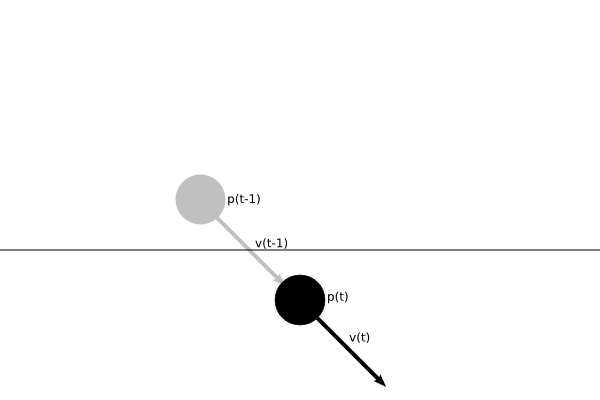
\includegraphics[width=0.4\textwidth]{graphics/Phys_kh1.png}}
			%\subfigure(2){
\includegraphics[width=0.4\textwidth]{graphics/Phys_kh2.png}}
			%\subfigure(2){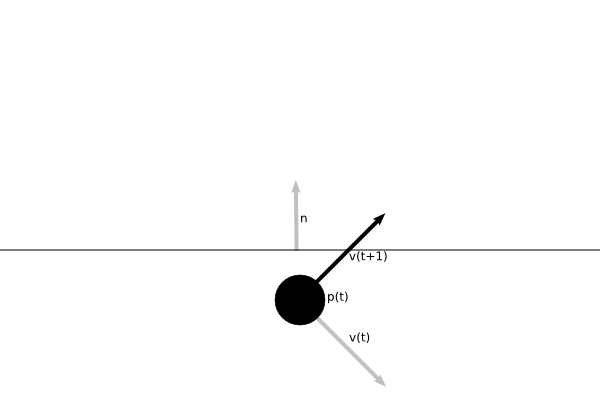
\includegraphics[width=0.4\textwidth]{graphics/Phys_kh3.png}}
			%\subfigure(2){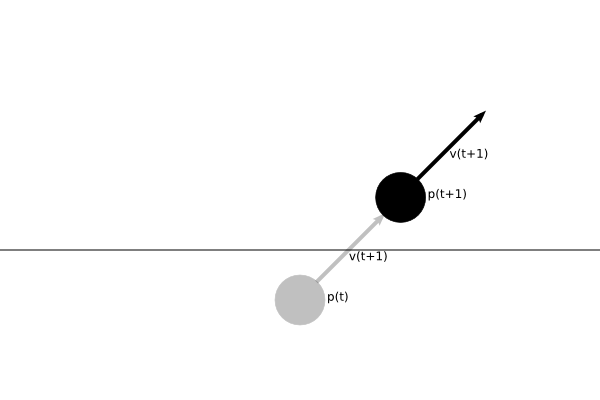
\includegraphics[width=0.4\textwidth]{graphics/Phys_kh4.png}}}
			
\includegraphics[width=0.99\textwidth]{graphics/Phys_kh1234.png}
			\caption{(1) Partikel dringt in die Heightmap ein. (2) Erkennung der Kollision. (3) Reflektion des Bewegungsvektors(v) entlang der Flächennormale(n). (4) }
			\label{fig:reflexHeihtmap}
		\end{figure}

		Allein mithilfe der Reflektion können bereits die meisten Kollisionen
		aufgelöst werden. Wenn beispielsweise ein Partikel senkrecht zur Oberfläche
		in die Heightmap eindringt wird der Bewegungsvektor auf diese Weise umgekert
		und das Partikel wird sich in der nächsten Iteration wieder aus der Heightmap
		herausbewegen.
		%\[ \vec{v}_{i}(t) = \left(\begin{array}{rr} 0 \\ 0 \\0 \end{array}\right) , \vec{f}_{i} = \left(\begin{array}{rr} 0 \\ -1 \\0 \end{array}\right) , \vec{n} = \left(\begin{array}{rr} 0 \\ 1 \\0 \end{array}\right) \]
		%\[ \vec{v}_{i}(t+1) = \left(\begin{array}{rr} 0 \\ -1 \\0 \end{array}\right) -2 \cdot \langle \left(\begin{array}{rr} 0 \\ -1 \\0 \end{array}\right) , \left(\begin{array}{rr} 0 \\ 1 \\0 \end{array}\right) \rangle \cdot \left(\begin{array}{rr} 0 \\ 1 \\0 \end{array}\right) = \left(\begin{array}{rr} 0 \\ 1 \\0 \end{array}\right) \]
		\\Die Kombination aus Reflektion und Gravitation führt außerdem dazu, dass
		Partikel die auf der Heightmap liegenbleiben sind, sich entlang des Gefälles
		der Heightmap bewegen, oder im Falle einer horizontalen Ebene auf der aktuellen Position liegenbleiben.
		Dies wird dadurch verursacht, dass ein liegengebliebenes
		Partikel einen Nullvektor als Bewegungsvektor besitzt, wodurch nach Verrechnung der
		Gravitation der Bewegungsvektor dem Vektor der Gravitation entspricht und
		verursacht dass das Partikel in die Heightmap bewegt wird, wodurch eine Kollision hervorgerufen wird.
		Wenn die Flächennormale in die entgegengesetzte Richtung der Gravitation
		zeigt, wie es im Fall einer horizontalen Ebene vorliegt, wird der
		Bewegungsvektor durch die Reflektion vollständig umgekehrt.
		In der nächsten Iteration wird das Partikel wieder an seine
		Ursprungsposition bewegt und die Addition der Gravitation zum Bewegungsvektor führt zur
		Neutralisierung der Bewegung, wodurch der Bewegungsvektor wieder
		zu einem Nullvektor wird und somit die Ausgangssituation wiederhergestellt ist.

		Wenn allerdings die Kollision an einem Gefälle stattfindet, neutralisieren
		sich Bewegung und Gravitation nur teilweise. Da die Gravitation keinen
		Einfluss auf den horizontalen Anteil der Bewegung hat, bleibt dieser
		erhalten und das Partikel bewegt sich in der nächsten Iteration in die
		horizontale Richtung der Flächennormale.
		Auf diese Weise bewegen sich Partikel auf der Oberfläche der Heightmap
		und folgen dabei der horizontalen Richtung der aktuellen Flächennormale.
		Bei einem Gefälle führt dieser Vorgang dazu, dass die Partikel sich,
		wie in Abbildung \ref{fig:rolling} dargestellt ist,
		entlang der schiefen Oberfläche nach unten bewegen, bis sie schließlich
		in einem Tal liegenbleiben. Oder im Fall einer horizontalen Ebene auf der Oberfläche liegenbleiben.
		\begin{figure}[h!]
			\centering
			\vspace*{30px}
			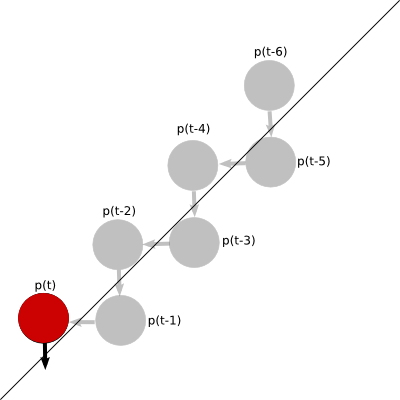
\includegraphics[width=0.7\textwidth]{graphics/Phys_rolling.png}
			\caption{Bewegung eines Partikels entlang eines Gefälles.}
			\label{fig:rolling}
		\end{figure}


		Nach der Reflektion kann die Reibung einbezogen werden, indem der Bewegungsvektor
		$\vec{v}_{i}$ von dem Reibungskoeffizienten $\mu$ gekürzt wird. Wobei $\mu$
		einen festen Wert zwischen 0 und 1 besitzen muss und für alle Partikel gleichermaßen gilt.
		\[ \vec{v}_{i}(t+1) = \vec{v}_{i}(t+1) \cdot ( 1 - \mu ) \]
		Bei dem Wert 1 würde das Partikel alle Bewegungsenergie verlieren und auf der
		Aufprallstelle liegenbleiben. Je kleiner dieser Wert jedoch ist desto weniger
		Energie geht bei einer Kollision verloren und ein Wert von 0 führt dazu, dass
		die Reibung keinen Einfluss mehr auf den Bewegungsvektor hat.

		Die Reibung sorgt dafür, dass die Partikel bei jeder Kollision immer langsamer
		werden, bis sie schließlich vollständig zum erliegen kommen und
		nicht dauerhaft ungebremst und durch die gesamte Welt springen.
		Der Verlust von Bewegungsenergie bedeutet allerdings auch, dass bei einem auf der
		Landschaft liegengebleibenes Partikel die Reflektion nicht mehr vollständig die
		Gravitation ausgleichen kann. Der Bewegungsvektor würde in der
		nächsten Iteration entgegen der Gravitation zeigen, dieser ist allerdings durch die Reibung
		schwächer als die Gravitation und kann diese nun nicht mehr vollständig neutralisieren. Die Reflektion
		reicht nun durch die Kombination mit der Reibung, nicht mehr alleine aus
		um zu verhindern, dass liegengebliebe Partikel immer weiter in die Oberfläche eindringen.

		Um dies zu verhindern wir ein weiterer Mechanismus bei der Kollisionsauflösung benötigt.



    \subsection{Kollisionserkennung zwischen Partikeln}
    	Um eine Kollision zwischen zwei Partikeln festzustellen errechnet man
    	den Abstand zwischen beiden indem man beide Positionsvektoren voneinander
    	subtrahiert und den Betrag des daraus resultierenden Vektors ermittelt.
    	Wenn alle Partikel kugelförmig sind und den gleichen Durchmesser besitzen
    	lässt sich eine Kollision sehr einfach ermitteln indem man den Abstand
    	zwischen den Partikeln mit dem doppelten Radius der Partikel vergleicht.
    	\[ \vert \vec{p}_{i} - \vec{p}_{j} \vert \leq 2r \rightarrow \textrm{Kollision liegt vor} \]
    	\[ \vert \vec{p}_{i} - \vec{p}_{j} \vert > 2r \rightarrow \textrm{Keine Kollision} \]
    	Solange der Abstand zwischen beiden Partikeln größer ist als der
    	doppelte Radius liegt keine Kollision vor.
    \subsection{Kollisionsauflösung zwischen Partikeln}
    	Wenn eine Kollision zwischen Partikeln festgestellt wurde, kann diese in
    	ähnlicher Weise aufgelöst werden wie eine Kollision mit der Landschaft.
    	Dabei
    \subsection{Übertragung der Kräfte zwischen Partikeln}
\end{Spacing}
\newpage
\clearpage
%% End Of Doc

\clearpage
% !TEX root = ../report.tex
\section{Die Benutzeroberfläche}
\begin{Spacing}{\mylinespace}

Nachdem die Grundfunktionalität der Hauptkomponenten unseres Systems standen ging es nun daran eine einfache aber dennoch funktionale Benutzeroberfläche zu entwerfen. Da das \textit{XNA-Framework} von Haus aus auf \textit{Windows-Forms} zur Darstellung von Benutzeroberflächen setzt, beschlossen auch wir vorerst diese Variante zu nutzen. Hielten uns aber die Möglichkeit offen eventuell später auf das etwas modernere \textit{WPF}-System zu wechseln.
\\\\
Hauptanforderungen waren ein übersichtliches Design und ein einfaches Hinzufügen von neuen Funktionalitäten. Um diese Anforderungen zu erfüllen entschieden wir uns für eine schlichte Statusleiste am unteren Rand des Editor-Fensters für einfache Anzeigen wie zum Beispiel die Frames Pro Sekunde(FPS) oder die Anzahl der Partikel und ein Tab-Panel an der rechten Seite des Editor-Fensters zur Konfiguration der einzelnen Komponenten. Durch die Nutzung des Tab-Panel lässt sich eine gute Separierung der einzelnen Komponenten in der Benutzeroberfläche realisieren. 
\\\\
Die Kommunikation zwischen der Benutzeroberfläche und den einzelnen Komponenten ist über das im \textit{.Net-Framework} integrierte Event-System realisiert. Bei einer Interaktion mit der Benutzeroberfläche wird ein entsprechendes Event gefeuert, welches anschließend die benötigten Daten an alle Komponenten liefert, die sich zuvor für dieses Event registriert haben.  

\begin{figure}[h!]
	\vspace*{30px}
	\includegraphics[width=\columnwidth]{graphics/gui.png}	
	\caption{Die GUI}
	\label{fig:GUI}
\end{figure}

\end{Spacing}
\newpage


\section{Properties}
Um unser System so dynamisch wie möglich zu gestalten entschlossen wir uns Sammelcontainer für Systemparameter einzuführen - sogenannte Properties.
Diese Properties lassen sich als Konfigurationsdateien ansehen. Ändert man einen Wert innerhalb einer Properties so wird er neue Parameter vom System sofort als neuer gültiger Wert angesehen.
Dadurch das jegliche Parameter einer Kategorie (Physikengine,RenderEngine,Kinect..) mit solch einer Properties ausgestattet sind, ist es möglich für verschiedene Anwendungscenarien Default-Wert zu hinterlegen und diese bei Bedarf zu laden oder zu speichern.

\section{Reflection}
Im Laufe der Zeit wurde unser Projekt immer größer, dies brachte auch viele neue Funktionalitäten mit sich.
All diese neuen Features mussten wir stetig unserer GUI-Oberfläche hinzufügen. Dieser sehr statische Ansatz wurde deshalb durch Reflektion in einen dynamischen überführt.
Diverse moderne Programmiersprachen so auch unser verwendetes C-Sharp besitzen die Möglichkeit während des Programmablaufs Informationen über die Struktur eines gegebenen Objekts abzurufen.

\begin{figure}[h!]
	\vspace*{30px}
	
\includegraphics[width=\columnwidth]{graphics/reflection.png}	
	\caption{Reflection}
	\label{fig:Reflection}
\end{figure}

Dieser Ansatz und die Tatsache das wir diverse Probleme mit unserer statischen Multi-Window GUI hatten, haben uns dazu bewegt unser altes GUI-System abzulösen.
Dank unseren Properties war es uns mittels Reflection möglich ein neues dynamisches GUI System einzuführen, hierbei verzichteten wir auch auf das Multi-Window System und haben die GUI direkt auf den Sandkasten projeziert.


\clearpage
%% End Of Doc
\clearpage

\end{Spacing}
\newpage
\clearpage
%% End Of Doc
\clearpage
% !TEX root = ../report.tex
\chapter{Ergebnisse}
\begin{Spacing}{\mylinespace}

hier schreiben wir unsere erfahrungen rein undwas wir genau hinbekommen haben. zudem sollen probleme die währed der arbeit aufgetreten sind erwähnt / erläutert werden. \\

\begin{figure}[h!]
	\vspace*{30px}
	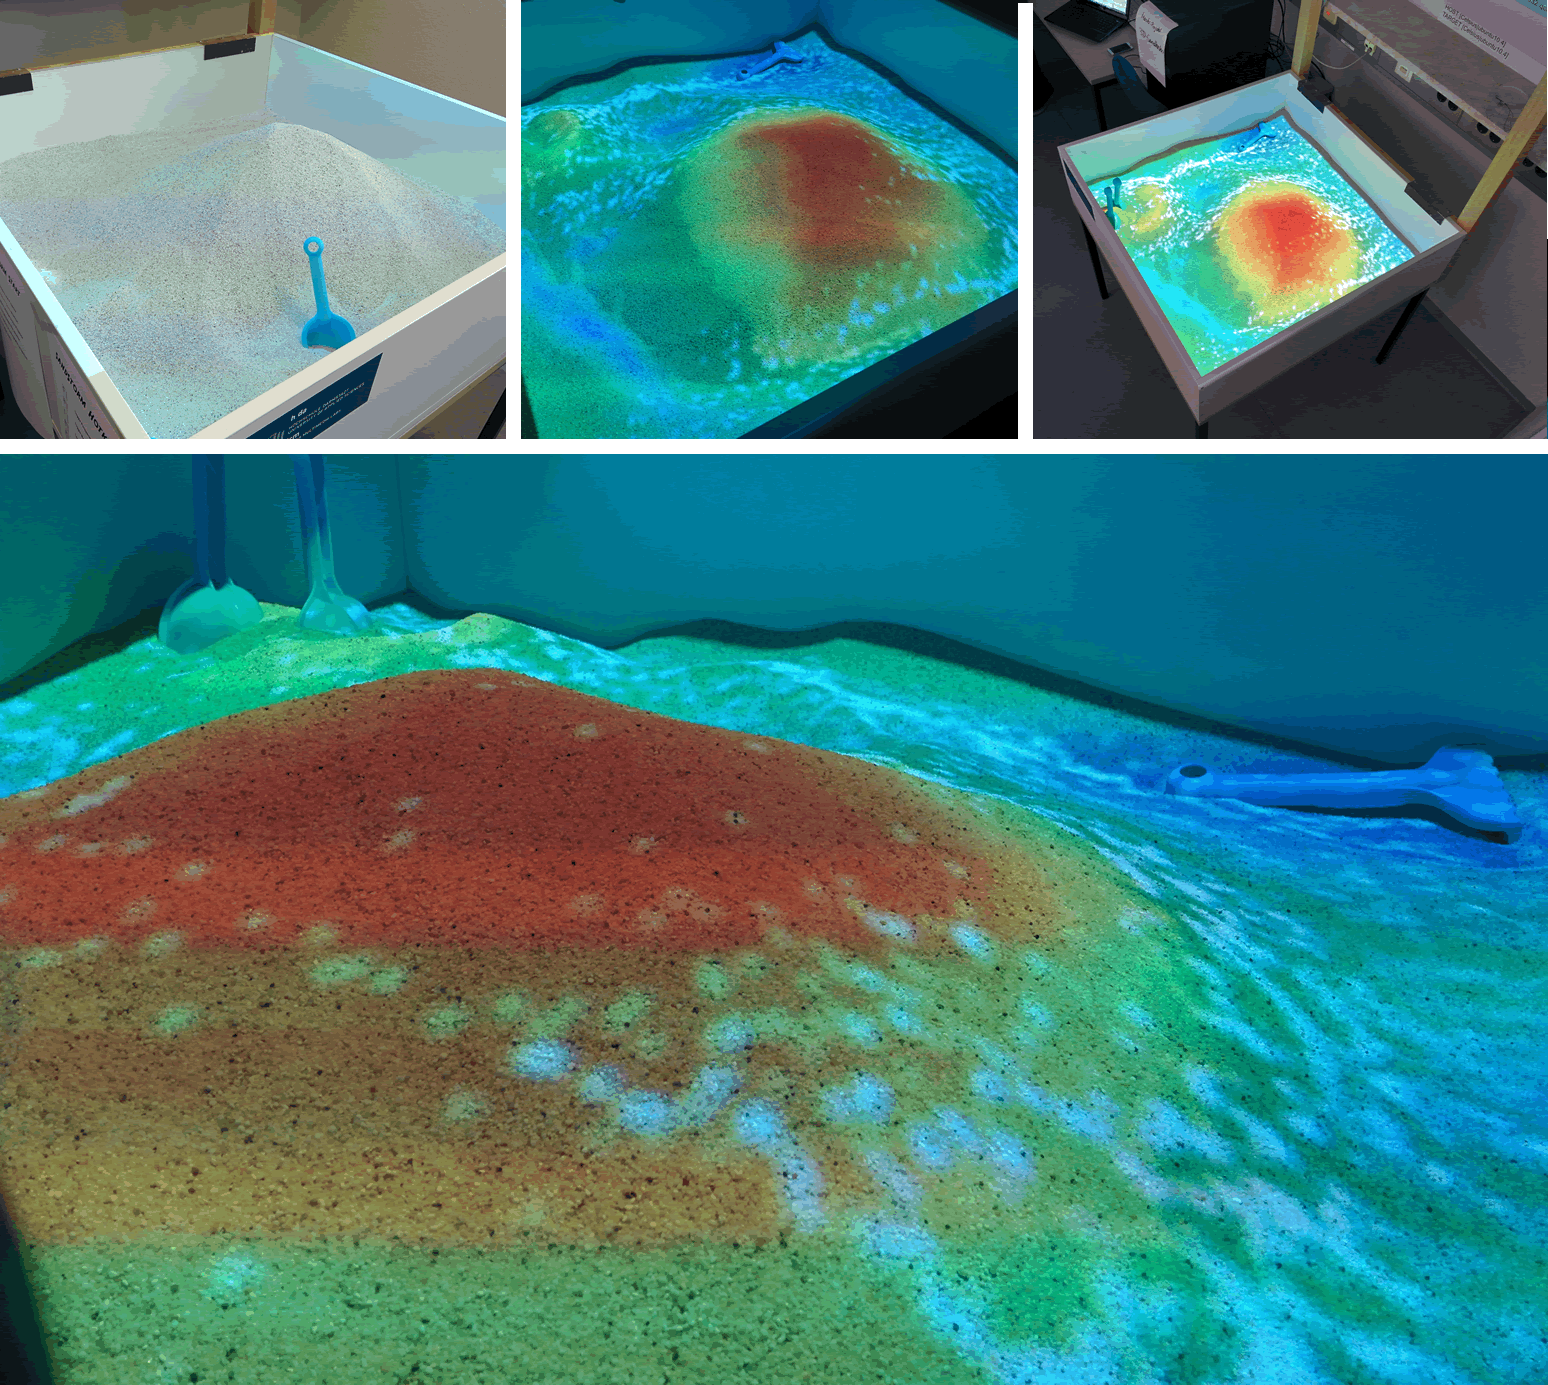
\includegraphics[width=\columnwidth]{graphics/results.png}	
	\caption{Sandstorm Projekt in Aktion.}
	\label{fig:Results}
\end{figure}

\end{Spacing}
\newpage
\clearpage
%% End Of Doc
\clearpage
% !TEX root = ../report.tex
\chapter{Probleme}
	\begin{Spacing}{\mylinespace}
	\section{Echtzeitfähigkeit}
	
		Leider besitzt die derzeitige Ausarbeitung diverse kleinere Probleme, welche die Echtzeitfähigkeit des Systems gefährden.
		Diverse teile von Berechnungen werden noch wie in \ref{physik} beschrieben auf der CPU ausgeführt, während der Teil der Visualisierung bereits auf die GPU portiert wurde.
		Dies führt zu erheblichen Performanceproblemen, denn es muss bei jeder Physikberechnung (jeden Frame), die Partikeldaten zwischen GPU und CPU kopiert und synchronisiert werden.
	\section{Darstellung}
		Die Darstellung stellte sich um Laufe des Projektes als schwieriger heraus als vorher angedacht.
		Hierbei kann man die Probleme auf welche wir gestoßen sind grob in Hard- und Softwareprobleme unterscheiden.
		\subsection{Hardware}
			Trotz das wir einen Beamer von einem Grafiklabor der Hochschule zur Verfügung gestellt bekommen haben, bemerkten wir bereits bei ersten Tests, das ein großer Farbunterschied zwischen Beamer und
			Monitor vorhanden ist. Leider scheint das Spektrum unseres Beamers sehr begrenzt zu sein, so das wir einen Farbunterschied zwischen weiß und gelb kaum wahrnehmen können.		
		\subsection{Software}
			Durch die physikalische Gegebenheit das Kinect und Beamer sich an unterschiedlichen Orten befinden, entsteht bei der Projektion zusätzlich zur Verzerrung auch noch das Problem der Verschiebung.
			Die Kalibrierung stellte sich somit schwieriger heraus als bisher gedacht, deshalb wurden aus zeitlichen Gründen der Fokus auf andere Aufgaben gesetzt um schnellstmöglich eine lauffähige Version zu erstellen.
	
\end{Spacing}
\newpage
\clearpage
%% End Of Doc
\clearpage
% !TEX root = ../report.tex
\chapter{Fazit \& Ausblick}

\begin{Spacing}{\mylinespace}
Trotz das auf uns allerlei Probleme zukamen, entstand im Laufe eines Semesters eine Echtzeit Sandkastensimulation, die bereits grundlegende Funktionalität bietet. 
Das Projekt wurde im  im Laufe des zweiten Semesters grundlegend neu strukturiert und somit anfängliche Performance Probleme erheblich verbessert.
Nicht nur auf die Erweiterbarkeit (Properties) wurde sehr hohen Wert gelegt sondern es wurden viele neue zusätzliche Parameter unserer Engine hinzugefügt.
Trotz der Tatsache, das man während der Entwicklung sehr schnell auf viele neue Ideen kommt, die man leider dann doch Aufgrund von Zeitmangel garnicht alle umsetzen kann haben wir uns nicht unterkriegen lassen und so viel es ging umgesetzt. Durch diverse DirektX-9 Probleme stoßen wir jedoch - wie bereits erwähnt, relativ schnell an die GPU-Grenzen des XNA-Frameworks.
Eine Neuprogrammierung haben wir jedoch ausgeschlossen - denn es musste eine stabile lauffähige Version bis zum Start der Hobit fertig gestellt sein.
Sollte jedoch in der Zukunft eine Neuprogrammierung in Frage kommen, wären zwei Wege denkbar.
Der erste Weg welcher es erlaubt einen Großteil des Codes wiederzuverwenden besteht darin das XNA Framework (DirectX 9) durch ein Upgrade von DirectX 10 oder gar 11 abzulösen.
Hierbei sollten die entstandenen Probleme mit DirectX9 behoben sein und es besteht die Möglichkeit durch diverse DirectX10/11 Wrapper für C\# mit der gleichen Sprache weiterzuarbeiten ohne das eine komplette Neuimplenetierung auf C++ nötig ist.
Der zweite aufwändigere Weg ist die Wahl von OpenGL, hierbei wird es nötig sein einen großteil des Codes von C\# auf C++ zu portieren und diverse Anpassungen der ShaderProgramme durchzuführen. Der große Vorteil - neben der Plattformunabhängigkeit, besteht darin das OpenGL derzeit bereits das Shader Model 5.0 sowie Compute-Shading anbietet was einen erheblichen Performance Zuwachs bieten sollte. Nachteil wäre jedoch, das dieser Weg ohne Vorkenntnisse im Bereich der GPU-Programmierung sehr zeitintensiv sein wird.
Dieses Projekt beinhaltet sehr viele Möglichkeiten und sollte in der Zukunft fortgeführt werden, jedoch benötigt es einen sehr großen Aufwand an Einarbeitungszeit deswegen wäre es schön wenn zukünftige Fächer der Hochschule bereits Grundlegende Kenntnisse im Bereich der GPU-Programmierung legen könnten.
	
\end{Spacing}
\newpage
\clearpage
%% End Of Doc
\clearpage
% !TEX root = ../report.tex
\appendix
\addtocontents{toc}{\setlength\cftchapternumwidth{1em}}

\begin{Spacing}{\mylinespace}
	\renewcommand\thechapter{}
	\chapter{Anhang}
	\renewcommand{\thechapter}{A}
	
	\section{Inbetriebnahme}
	\section{Hotkeys}
	
\end{Spacing}
\newpage
\clearpage
%% End Of Doc
\clearpage
 %and so on
%\inputTikZ{graphics/hardware}
%% end of doc
\clearpage

\pagenumbering{Alph}

\newpage
\printbibliography

%\newpage
%\listoffigures
%\newpage

%%%Anhang
%\appendix
%\renewcommand{\appendixtocname}{Anhang}
%\renewcommand{\appendixpagename}{\textsf{Anhang}}

%\appendixpage

\end{document}
